% begin module horizontal-asymptote-def
\begin{frame}
\begin{definition}[Horizontal Asymptote]
The line $y = L$ is called a horizontal asymptote of $f$ if either
\[
\lim_{x\to \infty}f(x) = L \qquad \text{ or } \qquad \lim_{x\to - \infty} f(x) = L.
\]
\end{definition}
\begin{itemize}
\item<2->  For example, $y = 1$ is a horizontal asymptote for $f(x) = \frac{x^2-1}{x^2+1}$.%
\item<3->  Can a function have two horizontal asymptotes?  \alert<handout:0| 4>{\uncover<4->{Yes.}}%
\end{itemize}
\uncover<4->{%
\psset{xunit=0.5cm, yunit=0.5cm}
\begin{pspicture}(-12,-2.5)(12,3.5)
\psaxes[ticks=none, labels=none]{<->}(0,0)(-10,-2.5)(10,3.5)
%Function formula: (3/2+1/2 ((x) (x))+2 (x))/((x)^{2}+1)+(- (2^{- (x)})+2^{x})/(2^{- (x)}+2^{x}) 
\psplot[linecolor=red, plotpoints=1000]{-12}{12}{2 x exp 2 x -1 mul exp -1 mul add 2 x exp 2 x -1 mul exp add div x 2 mul x x mul 0.5 mul add 1.5 add 1 x 2 exp add div add }
\rput(2.2, 3){$y=f(x)$}
\psline[linestyle=dashed, linecolor=blue](-12, -0.5)(12, -0.5)
\rput[t](10, -0.6){$y=y_0$}

\psline[linestyle=dashed, linecolor=blue](-12, 1.5)(12, 1.5)
\rput[b](-10, 1.6){$y=y_1$}
\end{pspicture} 
%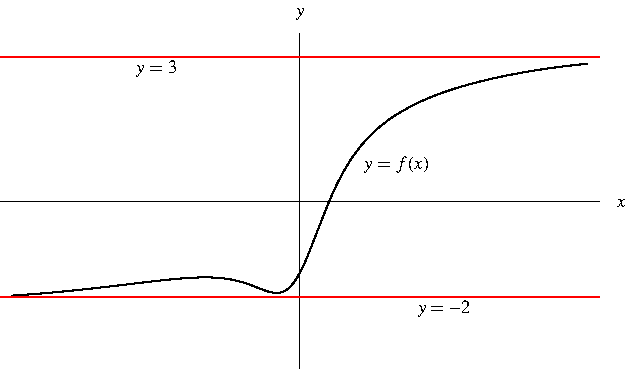
\includegraphics[width=8cm]{curve-sketching/pictures/04-04-twoasymptote.pdf}%
}%
\end{frame}
% end module horizontal-asymptote-def